\section{Introduction}
\label{sec:intro}

Energy consumption due to buildings (both residential and commercial)
is estimated to be 20\% to 40\% of the total energy usage in
developed countries~\cite{pop08}, and
lighting and heating are two significant components of this demand~\cite{keh05}.
Natural light (i.e., sunlight) is a readily available resource that
can contribute both to the illumination~\cite{Leslie03}
and to the heating~\cite{Lunde80} of structures,
yet in the vast majority of circumstances, its use is limited to
passive modalities.  For example, \emph{daylighting} (the use of natural
light for illumination) design is dominated by passive window positioning
and configuration~\cite{vgf+13} rather than active control mechanisms,
except in a few cases~\cite{kt16}.
Heating systems that exploit sunlight frequently use actively-controlled mirrors
for tracking the relative position of the sun, but there is limited experience
with using the same sets of mirrors for both thermal and lighting control.

We propose to investigate how to utilize actively
controlled catoptric (mirror) surfaces effectively for improved illumination and
heating of buildings.  Through computer-based control of the dynamic positioning of
individual mirrors, and cyber-physical integration of the mirrors, the devices
that orient them, and customized lighting and heating objectives and constraints,
we propose to enable fine-grained management of sunlight as a resource throughout
a building.

Figure~\ref{fig:amp} shows a prototype catoptric surface (called AMP) that was 
designed, fabricated, and installed during an undergraduate architecture studio 
taught by Co-PI C.~Ahrens. The installation redirects light from gable ends of an 
existing building into the darker recesses of the atrium to create better natural 
lighting where it is desired. In that installation, however, the mirror positions 
are fixed.

\begin{figure}[ht]
\centering
\subfloat[\mbox{ }]{

\includegraphics[width=0.5\linewidth]{figures/amp}
\label{fig:amp}}
\qquad \qquad
\subfloat[\mbox{ }]{
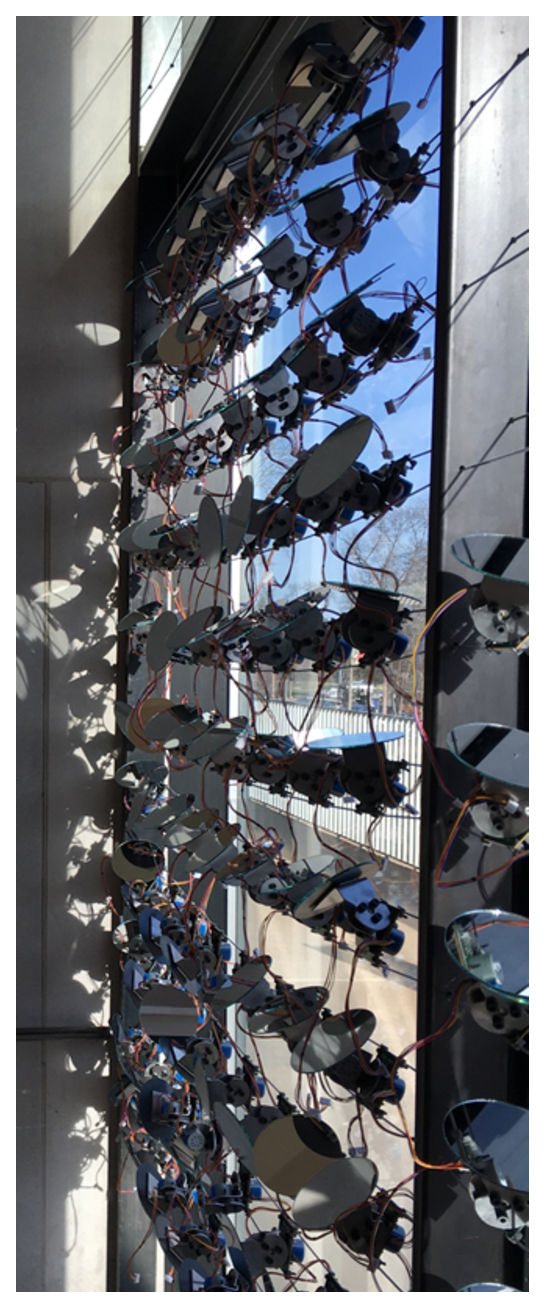
\includegraphics[width=0.16\linewidth]{figures/steinberg}
\label{fig:steinberg}}
\caption{Catoptric system prototypes.
(a)~\emph{AMP}, TRex building, St.~Louis.
(b)~Steinberg Hall, St.~Louis.
}
\label{fig:proto}
\end{figure}

Based on that fixed design, we are now developing a transformative 
new version of this approach in which over 600 mirrors are under 
active, 2-axis, microprocessor-based control and therefore the mirrors
can be pointed in different directions dynamically as desired over time. 
This next-generation installation is currently under construction within 
the south wall of the Steinberg Hall atrium on the Danforth Campus of 
Washington University in St. Louis): a subset of the mirrors in this new
installation is shown in Figure~\ref{fig:steinberg}.

The ability to control the position of each mirror actively and dynamically
offers an unprecidented capacity to direct available natural light to where
it is most needed.  The appropriate positioning of the mirrors can easily 
change over time, as the usage of the physical space changes, or as cloud
cover or temperature or other enviromental factors change.

Our proposed research will advance the state of the art in cyber-physical
management of reflected light, by allowing specific intensities to be achieved
in some areas while dissipated lighting conditions are achieved in other areas, 
according to pre-determined, yet adjustable, image-based maps. These maps may 
use any raster image to generate the target positions for the reflected light 
in a space.  
The image is sampled according to intensity (ranging from 
black to white) to determine the density of target points (the higher the 
intensity, the denser the resulting field of points. 

Using an image-based map 
also allows users of our system to visualize zones of intensity in an interior 
space prior to the mirrors reflecting the daylight. 
Users also will be provided interfaces for supplying or creating the images
to be used for the map, thus encouraging user-based control of, and
interaction with, the system. The engagement of any member of a community 
in the creation of that image in turn may impact on the entire community~\cite{BS13} 
and encourage dialog about the quality and quantity of light within the
environment. 

Given the desire to control natural light (sunlight) via a catoptric surface, and
also repurposing it for illumination and/or thermal management, a number of
cruicial cyber-physical systems issues must be addressed.
This research will investigate the following questions:
\begin{enumerate}

\item \emph{What are the qualitative and quantitative benefits
that can be achieved for bulding daylighting and thermal management
through the use of catoptric systems?}

Research challenges involved with this question include the ability to 
articulate different benefits, objectives, and constraints, and to quantify 
them effectively.  Clearly, doing so falls within the domain
of multi-objective control, so the relationships among potentially competing
goals also must be articulated and quantified. We intend to investigate
the use of Markov Decision Processes (MDPs) as an approach to
the multi-objective control problem, recognizing that maximization
(of an objective function) in expectation is a robust way to acknowledge
the inherent uncertainty of future events (whether it be sunlight availability,
lighting demand, or any other effect that is stochastic in nature).

\item \emph{How do we provide for the safety, reliability, maintainability, and
continued efficacy of these systems?}

Even with a suitable multi-objective control approach in place, the system as
a whole has limited usefulness if each requirement is not
addressed in an effective way.  For example, consider the question of
safety: highly concentrated sunlight aimed at a heat collector (important
when harvesting energy for thermal management purposes) could be harmful
to a person who inadvertently contacted the beam of light. 

Each system-level requirement thus must be included appropritely within
the control problem formulation, either as constraints (e.g., for
safety) or as additional objectives (e.g., reliability and/or maintainability).
Fortunately, the MDP formalism is well suited to the addition and integration 
of concerns such as these (especially those with a stochastic nature, as reliability
and maintainability tend to be).

\item \emph{Can we design abstractions that encapsulate subsystems for
effective reuse?}

Separating the concerns of low-level control (e.g., of mirror positions) from
the concerns of high-level system management (how the available light resource 
should be  allocated) is one way to approach this question.  The low-level control 
subsystem can be encapsulated into reusable components that may be applicable to 
any number of physical positioning applications, and that can be substituted as
needed to address new design constraints that may emerge for an installed catoptric 
system over time.  Similarly, high-level management components (e.g., based on 
different MDP models) also can be encapsulated, in a manner that allows them to be 
re-used in different kinds of cyber-physical systems or substituted to address 
different combinations of constraints and objectives within an installed system 
as its requirements evolve.

\end{enumerate}

\noindent
{\bf About us:}
Our group is uniquely qualified to address the questions we pose above.
We have significant expertise in the areas of computer engineering, architecture, 
and computer science that are relevant to this proposed research. We are already 
collaborating as an integrated team~\cite{cag18}, with one prototype system 
completed and installed and a second nearing completion.  We also have significant 
experience building cyber-physical systems~\cite{cew18,wgl17} and collaborating in 
MDP-based design of multi-objective resource management~\cite{mgc16}.
Co-PI C. Ahrens serves on the Board of Directors for the
Association for Computer Aided Design in Architecture (ACADIA).
In the past two years, Co-PI C. Gill has served as both program
chair and general chair of the ACM/IEEE International
Conference on Cyber-Physical Systems (ICCPS) and is currently
serving as an Associate Editor for ACM Transactions on Cyber-Physical
Systems.
PI R. Chamberlain is co-author of an introductory text on computing
in the physical world~\cite{cc17}.
